\let\negmedspace\undefined
\let\negthickspace\undefined
\documentclass[journal]{IEEEtran}
\usepackage[a5paper, margin=10mm, onecolumn]{geometry}
\usepackage{tfrupee} % Include tfrupee package

\setlength{\headheight}{1cm} 
\setlength{\headsep}{0mm}     

\usepackage{gvv-book}
\usepackage{gvv}
\usepackage{cite}
\usepackage{amsmath,amssymb,amsfonts,amsthm}
\usepackage{algorithmic}
\usepackage{graphicx}
\usepackage{textcomp}
\usepackage{xcolor}
\usepackage{txfonts}
\usepackage{listings}
\usepackage{enumitem}
\usepackage{mathtools}
\usepackage{gensymb}
\usepackage{comment}
\usepackage[breaklinks=true]{hyperref}
\usepackage{tkz-euclide} 
\usepackage{listings}
\def\inputGnumericTable{}                                 
\usepackage[latin1]{inputenc}                                
\usepackage{color}                                            
\usepackage{array}                                            
\usepackage{longtable}                                       
\usepackage{calc}                                             
\usepackage{multirow}                                         
\usepackage{hhline}                                           
\usepackage{ifthen}                                           
\usepackage{lscape}
\usepackage{circuitikz}
\tikzstyle{block} = [rectangle, draw, fill=blue!20, 
    text width=4em, text centered, rounded corners, minimum height=3em]
\tikzstyle{sum} = [draw, fill=blue!10, circle, minimum size=1cm, node distance=1.5cm]
\tikzstyle{input} = [coordinate]
\tikzstyle{output} = [coordinate]


\begin{document}

\bibliographystyle{IEEEtran}
\vspace{3cm}

\title{3.4.5}
\author{AI25BTECH11036-SNEHAMRUDULA}
 \maketitle
{\let\newpage\relax\maketitle}
\renewcommand{\thefigure}{\theenumi}
\renewcommand{\thetable}{\theenumi}
\setlength{\intextsep}{10pt} 
\numberwithin{equation}{enumi}
\numberwithin{figure}{enumi}
\renewcommand{\thetable}{\theenumi}
\textbf{Question}:\\
\textbf{3.4.5} Construct a rhombus whose side is of length $3.4 \, \text{cm}$ and one of its angles is $45^\circ$.
\solution \\
%-----------------------------------------
% Q 3.4.5 : Rhombus construction (gvv methods)
%-----------------------------------------
Let the side length be 
\begin{align}
    s &= 3.4                                            \label{eq:rhomb1}
\end{align}
and the given angle be
\begin{align}
    \theta &= 45^\circ.                                 \label{eq:rhomb2}
\end{align}

\noindent
We now place the vertices of the rhombus as follows:
\begin{align}
    \vec{A} &= \myvec{0\\0},                            \label{eq:rhombA}\\
    \vec{B} &= s\myvec{1\\0},                           \label{eq:rhombB}\\
    \vec{D} &= s\myvec{\cos\theta\\ \sin\theta}.        \label{eq:rhombD}
\end{align}

\noindent
The fourth vertex is obtained using the parallelogram law:
\begin{align}
    \vec{C} &= \vec{B} + \vec{D} - \vec{A}.             \label{eq:rhombC}
\end{align}

\noindent
Thus, the coordinates of the rhombus are
\begin{align}
    \vec{A} &= \myvec{0\\0},                            \label{eq:rhombA2}\\
    \vec{B} &= \myvec{3.4\\0},                          \label{eq:rhombB2}\\
    \vec{D} &= \myvec{\tfrac{3.4}{\sqrt{2}}\\ \tfrac{3.4}{\sqrt{2}}}, 
                                                      \label{eq:rhombD2}\\
    \vec{C} &= \myvec{3.4+\tfrac{3.4}{\sqrt{2}}\\ \tfrac{3.4}{\sqrt{2}}}.
                                                      \label{eq:rhombC2}
\end{align}

\noindent
Verification of equal sides:
\begin{align}
    \norm{\vec{B}-\vec{A}} &= s,                        \label{eq:check1}\\
    \norm{\vec{D}-\vec{A}} &= s,                        \label{eq:check2}\\
    \norm{\vec{C}-\vec{B}} &= s,                        \label{eq:check3}\\
    \norm{\vec{C}-\vec{D}} &= s.                        \label{eq:check4}
\end{align}

\noindent
Hence, $ABCD$ is a rhombus with side length $s=3.4$ cm and $\angle DAB = \theta = 45^\circ$.


\begin{figure}[h!]
    \centering
    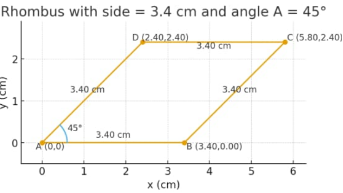
\includegraphics[height=0.4\textheight, keepaspectratio]{fig3.4.5}
    \label{figure_1}
\end{figure}
 
\end{document}